\documentclass[a4paper,11pt,twoside]{article}%
\usepackage[lmargin=90pt,rmargin=90pt,tmargin=127pt,bmargin=123pt]{geometry}
\usepackage[latin1]{inputenc}
\usepackage[frenchb]{babel}
\usepackage[table]{xcolor}
\usepackage{array}
\usepackage{graphicx}
\usepackage{caption}
\usepackage{subcaption}
\usepackage{listings} 
\usepackage{setspace}
\usepackage{amsthm}
\usepackage[section]{placeins} 
\usepackage{hyperref} % Cr�er des liens et des signets 
\hypersetup{	
colorlinks=true, %colorise les liens 
breaklinks=true, %permet le retour � la ligne dans les liens trop longs 
urlcolor= blue, %couleur des hyperliens 
linkcolor= black,	%couleur des liens internes 
citecolor=black,	%couleur des r�f�rences 
} 
\setstretch{1,3}
\frenchspacing
\usepackage{textcomp}
\title{Projet \\ TDLOG  }
\author{Quentin B�rard \and Valentin Berkes \and Fran�ois Dupr�}
\date{Janvier 2016}

\begin{document}

\begin{titlepage}

\begin{figure}[ht]
\centering

\includegraphics[width=0.4\linewidth,keepaspectratio]{ecole_ponts_rvb_transparent}
\vspace{40pt}
\end{figure}
	
		\centering
    {\LARGE Projet TDLOG\\  \vspace{25pt} \textbf{Kahmat\'e}} \\ \vspace{150pt}
    {\Large Quentin B\'erard \hspace{15pt} Valentin Berkes \hspace{15pt} Fran�ois Dupr\'e }\\
		\vfill
		 {\large	Janvier 2016}
\end{titlepage}



\section{Objectif initial}

Notre objectif initial fut de r\'ealiser un jeu de Kahmat\'e fonctionnel, et d'impl\'ementer une intelligence artificielle. Nous pensions d'abord en finir rapidement avec l'impl�men-tation du jeu, pour pouvoir ensuite nous consacrer pleinement \`a l'intelligence artificielle, la partie la plus difficile \`a encoder selon nous.


Le but \'etait donc d'abord fonctionnel : rendre un jeu qui marche. L'unique contrainte non-fonctionnelle que nous nous \'etions fix\'es : une certaine robustesse aux bugs. La performance, en revanche, n'est que peu rentr\'ee en ligne de compte, sauf lorsque nous avons pens\'e \`a faire une IA.

Dans l'esprit du cours de d\'eveloppment logiciel, nous n'avions pas de contrainte pr\'ecise quant au travail \`a accomplir : nous \'etions libres de faire les choix que nous souhaitions pour mener \`a bien notre travail.

En d\'efinitive, nous avions donc carte blanche pour accomplir notre but m\^eme si notre encadrant, Xavier Clerc, \'etait pr\'esent pour nous apporter son exp\'erience et ses conseils.

 
\section{Technologies mises en oeuvre}

Nous avons cod\'e notre jeu de Kahmat\'e en langage Python. Cela nous a grandement facilit\'e la t\^ache dans la mesure o\`u ce langage est d'un maniement relativement simple et intuitif, surtout lorsqu'on le compare \`a d'autres langages, comme le C.

\subsection{Sch\'ema du code}

\subsubsection{Fichier central}
 Il nous a ainsi \'et\'e facile d'organiser notre fichier principal, \textbf{projet.py}. Celui-ci se d\'ecompose principalement en quatre classes :
\begin{itemize} 
\item Une pour le ballon contenant les instances qui concernent le porteur et le d\'eplacement du ballon.\\
\item Une pour les joueurs o\`u se trouvent les m\'ethodes les plus importantes du jeu : celles pour d\'eplacer les joueurs (\textbf{deplace} et \textbf{deplacement}), pour plaquer (\textbf{placage}), pour passer en force, pour faire une passe et pour tirer en avant. \\
\item Une pour les \'equipes de facon \`a rassembler tous les joueurs d'une m\^eme \'equipe. \\ 
\item Une derni\`ere pour le jeu en lui-m\^eme, permettant de l'initialiser, de r\'esoudre les actions et de g\'erer le tour de chaque joueur. \\
\end{itemize}

\subsubsection{Fichiers annexes}
Autour du fichier central, \textbf{projet.py}, qui contient le coeur du jeu, nous avons ajout\'e de nombreux fichiers secondaires :
\begin{itemize}

\item Plusieurs fichiers pour r\'ealiser les tests, un pour l'interface graphique, un autre pour la gestion des queues et un dernier pour lancer le jeu. Nous voulions assurer une couverture de code maximale.
A cet \'egard, Python poss�de un grand nombre de biblioth\`eques qui se sont r\'ev\'el\'ees tr\`es utiles, en particulier celles relatives aux tests :
\begin{itemize}
\item \textbf{unittest} nous a permis de tester notre code et nos fonctions, notamment les principales m\'ethodes de la classe Joueur : \textbf{d\'eplace}, 
\textbf{d\'eplacement} et \textbf{placage}.
\item Le module \textbf{coverage} a permis de v\'erifier dans quelle mesure les nombreuses fonctions, correspondant \`a toutes les actions diff\'erentes, \'etaient bien parcourues par les tests.
\end{itemize}

\item Quant \`a l'interface graphique, nous avons utilis\'e des biblioth�ques telles que \textit{Threading} ou encore \textit{PyQt} pour construire notre jeu et faire en sorte que les actions r\'ealis\'ees avec la souris soient effectives : nous avons mod\'elis\'e les joueurs et leurs actions par des boutons cliquables. Il a donc fallu lier \`a chaque bouton un objet ou une m\'ethode.

\end{itemize}
\section{Gestion du projet}

Pour mener bien notre projet, nous avons utilis\'e divers outils de communication et de partage. 
\subsection{Github}

\begin{figure}[!h]
	\begin{center}
	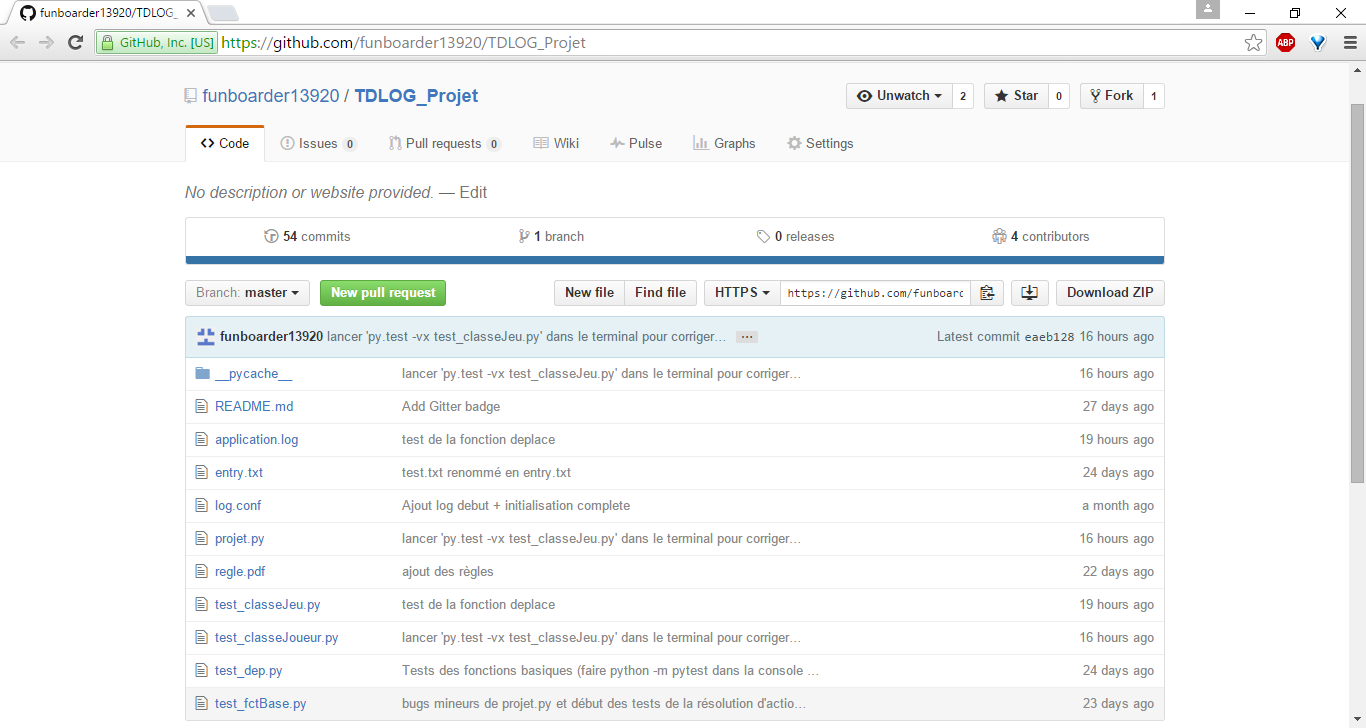
\includegraphics[scale=0.4]{github.png}
	\caption{GitHub du projet}
	\end{center}
\end{figure}

Pour g\'erer le partage du code de fa�on efficace, nous nous sommes servis de Github, une plate-forme permettant l'\'echange de fichiers. L'avantage de Github est qu'il permet � chacun de modifier librement le code fait par les autres sans que cela affecte la totalit\'e. Ensuite, il suffit de push pour partager les modifications effectu\'ees avec tous les autres aussit\^ot qu'ils feront un pull. De cette facon, la coordination entre nous s'est retrouv\'ee consid\'erablement simplifi\'ee car \`a chaque pull, c'est Github lui-m\^eme qui se charge d'int\'egrer automatiquement les nouveaut\'es. 

En cas de conflit, il le signale pour que l'utilisateur le r\`egle manuellement. Pour communiquer, nous avons bien \'evidemment \'echang\'e des mails, mais l'utilisation d'un tchat nous a vite paru indispensable, c'est pourquoi nous nous sommes tourn\'es vers Slack. 


\subsection{Slack}

\begin{figure}[!h]
	\begin{center}
	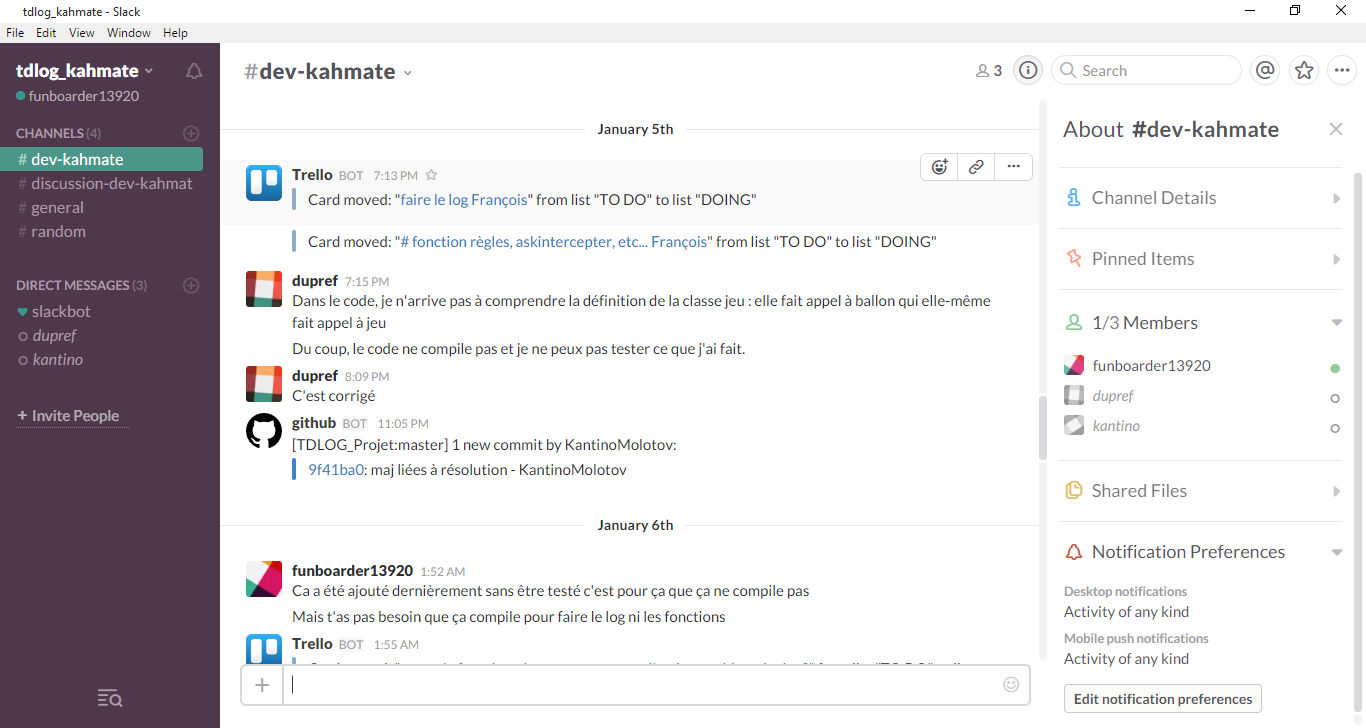
\includegraphics[scale=0.4]{slack.png}
	\caption{Slack du projet}
	\end{center}
\end{figure}

Slack nous a permis d'avoir des \'echanges plus efficaces et de dynamiser notre communication. Il devenait ainsi plus facile de demander de l'aide aux autres en cas de probl\`eme, de signaler ce qui ne fonctionnait pas ou encore d'indiquer les bugs qui venaient d'\^etre corrig\'es. Ce fut donc \'et\'e notre outil principal pour communiquer. Cette plate-forme avait de nombreux avantages, mais les messages pouvaient parfois d\'efiler tr\`es rapidement et la recherche d'un commentaire particulier devenait fastidieuse. C'est pourquoi nous avons aussi utilis\'e Trello qui nous a permis d'organiser plus ais\'ement les projets, afin de savoir plus clairement ce qui devait \^etre fait.


\subsection{Trello}

\begin{figure}[!h]
	\begin{center}
	\includegraphics[scale=0.4]{trello.png}
	\caption{Trello du projet}
	\end{center}
\end{figure}

Notre espace Trello \'etait constitu\'e :
\begin{itemize}
\item d'une premi\`ere liste montrant les bugs \`a r\'esoudre,
\item d'une deuxi\`eme indiquant ce qui restait \`a faire
\item d'une troisi\`eme indiquant ce qui \'etait en cours
\item d'une derni\`ere affichant ce qui avait \'et\'e fait.
\end{itemize}


De cette facon, il \'etait tr\'es simple de savoir ce que chacun \'etait en train de faire ou devait faire. Tout \'etait class\'e et la plupart des t\^aches portait le nom du membre du projet qui devait s'en charger. Nous avons choisi de mettre les bugs hors des autres listes car ils correspondaient souvent \`a des probl\`emes majeurs qui emp\^echaient le programme de fonctionner correctement et qu'il \'etait par cons\'equent n\'ecessaire de r\'esoudre au plus vite. 

\subsection{R\'epartition des t\^aches}
\begin{itemize}
\item Valentin a \'ecrit les tests, les classes du jeu, quelques fonctions du jeu et s'est en grande partie occup\'e de l'interface graphique.
\item Quentin s'est charg\'e d'\'ecrire les m\'ethodes principales (placage, deplace, deplacement) en essayant de trouver des compromis pour faciliter l'\'ecriture du code tout en respectant les r�gles du jeu. 
\item Francois a \'ecrit les log d'erreurs, comment\'e le code et organis\'e la r\'edaction du rapport.

\item Nous avons tous particip\'e au debug du programme suite aux tests. Lorsque les erreurs \'etaient simples \`a corriger chacun s'en occupait de son c\^ot\'e. \\
En revanche, lorsqu'il s'agissait d'une erreur dans le comportement d'une fonction, celui qui l'avait cod\'ee qui devait la r\'eviser. De cette mani�re, chacun avait des parties du code qu'il connaissait mieux que les autres et qu'il �tait le plus � m�me de corriger ou de modifier.

De plus, car les tests n'ont pas forc�ment �t� �crits par celui qui a cod\'e les m�thodes, ils ont \'et\'e r\'ealis\'es en bo\^ite noire (ou grise tout du moins). Ainsi, nos tests se sont trouv\'es \^etre plus diversifi\'es, et donc plus efficaces que si chacun avait cod\'e des tests pour les fonctions qu'il avait \'ecrites. 

\item Nous nous sommes aussi r\'eunis r\'eguli\`erement, d'abord chaque mercredi matin pendant le cours de TDLOG, mais aussi de plus en plus souvent en dehors de ce cr\'eneau au fur et \`a mesure que l'\'ech\'eance approchait. Cela afin de discuter de l'orientation que devait prendre le projet, notamment en ce qui concerne l'intelligence artificielle, l'interface graphique ou les interpr�tations possibles des r�gles du jeu.

\end{itemize}

\subsection{Organisation du groupe}

Il nous a rapidement sembl\'e plus judicieux de nous orienter vers une gestion de projet classique, plut\^ot que d'adopter les m\'ethodes qui nous avaient \'et\'e pr\'esent\'ees par Theodo, comme les gestions Scrum ou XP. En effet, au regard du faible nombre de personnes impliqu\'ees dans le projet (trois), et que la demande risquait assez peu d'\'evoluer au cours du projet, nous avons opt\'e pour une structure classique en V : d'abord, sp\'ecification et conception, puis correction des bugs par des tests de diff\'erentes natures. Il nous a sembl\'e que cette m\'ethode se pr\^etait plus \`a un projet simple comme celui-ci. En effet, le jeu a \'et\'e assez vite sur le point d'\^etre fini : au fur et \`a mesure de l'avanc\'ee du projet, les tests et le debuggage occupaient une partie de plus en plus importante de notre temps.


\section{Les probl\`emes rencontr\'es}

Au cours du d\'eroulement du projet, nous avons \'et\'e confront\'es \`a plusieurs difficult\'es 

\subsection{Manier de nouveaux outils : GitHub}

GitHub \'etait un outil nouveau pour nous tous. Il nous a fallu du temps pour bien le ma\^itriser. Par exemple, au d\'ebut, la proc\'edure \`a suivre lors d'un probl\`eme de fusion de fichiers apr\`es un pull ne nous a pas sembl\'e tr\`es intuitive. Ainsi, vers le milieu du projet, il y a eu de nombreuses confusions, surtout lorsque tout le monde faisait des push simultan\'ement. Il nous a donc fallu un peu de temps pour nous habituer \`a ce nouvel environnement de travail. 

\subsection{Kahmat\'e}
Ensuite, il y a eu des probl�mes avec le jeu en lui m\^eme. Nous avons parfois pris des d\'ecisions pour simplifier notre code tout en respectant les r\`egles du jeu. Par exemple, pour la fonction \textbf{placage}, le choix de la case o\`u le ballon doit arriver en cas de succ\`es n'est pas \'evidente. Nous avons choisi de le placer \`a l'oppos\'e du plaqueur avec des cas particuliers pour les bords du terrain. D'autres choix \'etaient possibles mais ils risquaient d'\^etre plus compliqu\'es \`a impl\'ementer et il fallait garder du temps pour produire l'interface graphique.

\subsection{L'intelligence artificielle}

En premi\`ere approche, nous souhaitions 
r\'ealiser, en sus du jeu simple, une intelligence artificielle contre laquelle un humain pourrait jouer.  Malheureusement, apr�s un change de mails avec un expert du domaine, Tristan Cazenave, nous avons choisi d'abandonner l'id\'ee de faire une IA car il s'av\`ere qu'elle aurait \'et\'e beaucoup trop lente. En effet, deux possibilit\'es qui s'offraient \`a nous :
\begin{itemize}
\item L'algorithme min-max , qui consiste, par l'interm�diaire d'une fonction d'\'evaluation et un algorithme arborescent, \`a minimiser les pertes d'un joueur en supposant que l'adversaire souhaite les maximiser. Malheuresement, cet algorithme demandait le calcul d'un minimum sur un nombre de coups (dit facteur de branchement) dont nous avons vite compris qu'il allait se r\'ev\'eler \^etre prohibitif (aux alentours de 1000, sachant que pour un jeu de Go, o\`u l'algorithme min-max ne fonctionne pas, il est aux alentours de 400). Nous avons un moment envisag\'e de r\'eduire artificiellement le facteur de branchement, en limitant le nombre de coups possibles pour notre IA, avant d'abandonner en constatant que le facteur de branchement serait toujours rest\'e trop \'elev\'e.
\item Les syst\`emes experts, qui consistent \`a pratiquer le jeu, et \`a r\'ealiser un algorithme ad hoc. En raison de la contrainte de temps, nous n'avons finalement pas pu choisir cette solution. 
\end{itemize}


Nous nous sommes donc concentr\'es sur l'interface graphique, qui, bien que plus chronophage, nous assurait un r\'esultat.


\subsection{Debugger}

La gestion de projet en V nous a \'et\'e assez b\'en\'efique pour ce programme. En effet, les diff\'erentes classes et m\'ethodes \'etaient imbriqu\'ees les unes dans les autres. Par cons\'equent, tout test unitaire \'etait impossible (ou presque). En premier lieu, nous avons donc pleinement mis \`a profit le concept de mock object.
Par la suite, nous avons pu repasser \`a des tests de niveau de granularit\'e plus \'elev\'es : par int\'egration ou par validation.

Nous avons rencontr\'e un certain nombre de r\'egressions, par exemple lors de la mise en place des logs. Ces r�gressions ont pu �tre corrig�es rapidement et efficacement gr�ce aux tests d�j� mis en place.

Depuis que l'interface graphique a \'et\'e int\'egr\'ee, il ne nous est plus possible de lancer les tests. En effet, nous lancions ces derniers depuis la version de notre jeu avec une interface utilisateur sur la console. Bien entendu, nous avons bien v\'erifi\'e que les fonctions r\'epondaient au cahier des charges avant de finalement les int\'egrer dans l'interface.


\subsection{R\`egles}

Nous nous sommes rendus compte que nous avions mal interpr�t� un point de d\'etail des r\`egles. En effet, l'utilisation de telle ou telle carte Forme, qui participe \`a la r\'esolution des actions, doit \^etre un choix du joueur et non pas le fait du hasard. Contraint par le temps, nous n'avons pas pu corriger cette interpr�tation qui selon nous n'emp�che pas le joueur de jouer et ne fait perdre aucune saveur au jeu.

\section{Les r\'esultats obtenus}

\subsection{Jouer}

Ainsi, il est possible de jouer au jeu int\'egralement avec la souris : au d\'ebut, le jeu nous invite \`a positionner les joueurs de chaque \'equipe. Pour cela, il suffit de cliquer sur le joueur puis sur la case o\`u on veut le placer. Ensuite, le jeu commence. Pour jouer, on clique une premi�re fois sur le joueur qu'on veut utiliser puis on clique sur une autre case.


En fonction de la case choisie, une action va se d\'eclencher : une passe si on clique sur un joueur en arri\`ere, un tir en avant si on clique sur une case devant le joueur et qui ne soit pas juste devant lui, un d\'eplacement si on clique sur une case voisine non occup\'ee ou un plaquage (ou passage en force) dans le cas contraire. Cette technique de programmation fonctionne car au plus une action peut \^etre r\'ealis\'ee suivant la case de notre second clique. En effet, notre m\'ethode deplacement a \'et\'e cod\'ee pour ne permettre de se d\'eplacer que d'une case la fois. De cette mani\`ere, un d\'eplacement et un tir en avant ne peuvent par exemple pas \^etre confondus.

En d\'efinitive, \`a la fin de la p\'eriode de d\'eveloppement, nous sommes parvenus \`a cr\'eer notre jeu de Kahmate.\\

\begin{figure}[!h]
	\begin{center}
	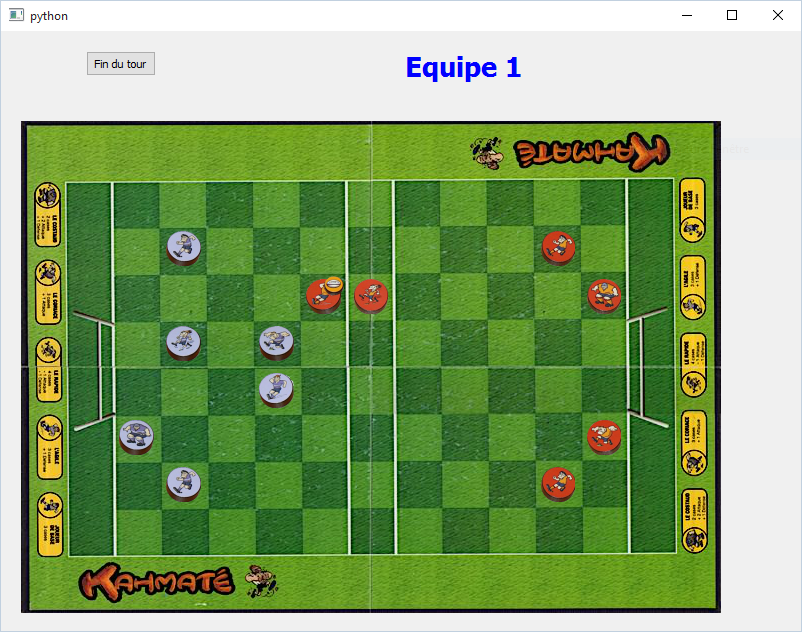
\includegraphics[scale=0.5]{kahamate.png}
	\caption{L'interface graphique de notre Kahmat�}
	\end{center}
\end{figure}


\subsection{Conclusion}
Notre jeu est op\'erationnel, il est possible d'y jouer \`a deux sur une m\^eme machine. Les fonctionnalit�s principales ont \'et\'e test�es plusieurs fois dans des cas distincts (test par \'enum\'eration, principalement) et semblent satisfaisantes. On peut enti\`erement jouer \`a la souris gr\^ace l'interface graphique.Il y a une divergence par rapport � ce qui \'etait pr\'evu au d\'epart puisque l'intelligence artificielle n'a finalement pas vu le jour, mais son absence a \'et\'e compens�e par une meilleure interface graphique. Cela mis \`a part, le r\'esultat final nous para\^it en accord avec ce que nous avions annonc\'e au d\'ebut.

\end{document}
